% !TeX root = ../main.tex
\chapter{考虑跨机资源竞争的无人机集群截止期优先计算任务分配}
\label{cha:fixed-offload}

\section{问题描述与跨机迁移外部性分析}
\label{sec:ch4-problem-externality}

第三章解决无人机集群通过空间部署接纳地面需求的问题，本章进一步研究已接纳计算任务在集群内部如何分担。请求接入某架无人机后，其执行节点仍可选择来源本机、允许的协作无人机或地面 MBS；本章沿用由 5 架无人机与 1 个地面 MBS 构成的六节点服务系统。执行位置会改变回源、机间转发、机载计算负载和能耗，因此跨机任务分配不仅涉及为单个请求选择最快节点，还涉及选择后整批请求如何分享各机算力：一项迁移可能使目标请求提前完成，也可能同时使迁入节点上多个原有请求超时。

这里的任务分配以不可拆分的计算请求为对象，关联无人机承担接纳与上传职责，执行节点承担计算职责。二者可以不同，因而集群具有在空间接入后继续协作分工的机会。不同无人机的算力、缓存与链路条件不同，地面 MBS 则作为六节点服务系统中的强算力支撑。本章保持这些既有资源规则，研究任务从一个执行节点转移到另一个节点时的系统后果；这与为飞行器分配巡检航点、侦察目标或编队位置具有不同的任务语义。

为在可控条件下比较不同分配方案，本章采用固定快照与反事实评价协议。固定快照指将某一时隙的 UAV 与 UE 历史几何、当前缓存、电量、请求集合及配置整体冻结；反事实评价指同一快照上的各候选分配均从完全相同的初始状态出发，由仿真环境执行整批请求，得到完成时延与 UAV 分配能耗。候选执行结果不回写采样所用的参考历史，下一快照仍取自同一参考控制轨迹。该受控设计将“执行目标选择差异”与“历史演化导致的状态差异”解耦，使候选分配之间具备直接可比性。固定快照下的研究问题为：在自然接纳与最终批量负载均分的条件下，以最小化超时请求数为首要目标的跨节点迁移搜索，能否较仅依据单请求自身代价的启发式获得更优的集群当步分工，以及该质量余量所需的能耗与求解时间代价。本章方法由此为集群任务分配提供受控分析框架，并在相同快照上给出可达分配质量的上界参照；第五章在此基础上构建在线下层，以配额搜索与条件匹配在有限决策预算内逼近上述质量参照。

\subsection{固定快照反事实评价模型与决策变量}
\label{sec:ch4-variables}

记当前接纳的服务请求集合为 $\mathcal M$，请求总数为 $K=|\mathcal M|$。地面 UE 总数记为 $M$，活跃请求由其在当前时隙泊松或流行度到达生成。每个请求 $m$ 包含来源 UAV $u_m$、请求数据量 $L_m$、计算程序镜像大小 $B_{s_m}$、所需 CPU 周期数 $C_m=\omega_{s_m}L_m$ 以及硬性截止时间 $D_m$。每个请求的候选执行节点集合记为 $\mathcal C_m$，由来源本机、MBS 以及通信拓扑上允许的机间跳步邻居构成。整批任务分配决策向量记为 $\mathbf a=(a_1,\ldots,a_K)$，其离散决策空间定义为：
\begin{equation}
 \mathcal A=\prod_{m\in\mathcal M}\mathcal C_m,\qquad
 |\mathcal A|=\prod_{m\in\mathcal M}|\mathcal C_m|.
 \label{eq:ch4-assignment-space}
\end{equation}
当某协作节点的转发拓扑不可达、链路处于深衰落、目标机当前电量不足以支撑回源或 MBS 回传链路中断时，对应候选执行分支被判定为不可行并从 $\mathcal C_m$ 中剔除。这使得候选空间在搜索之初便严格限定在硬件可行域之内。

在固定快照测试中，无人机与终端的空间几何构型、信道大尺度衰落及小尺度信噪比状态被严格冻结。请求上传时延 $U_m$、协作转发时延 $I_{m,u,v}$、回源传输时延 $V_{j,s}$ 以及各节点的本地缓存命中指示变量 $h_{j,s}\in\{0,1\}$ 均取自快照冻结值。每个候选执行路径的端到端时延仅取决于所选执行节点及其最终汇聚的并发任务负载。

\subsection{实际服务路径与端到端时延推导}
\label{sec:ch4-actual-paths}

给定分配决策向量 $\mathbf a$，请求 $m$ 的端到端时延随所选执行位置不同而由不同分量构成。若由来源本机执行（$\mathrm{local}$），时延由无线接入上传、未命中时的回源与机载计算三部分构成；若由协作无人机执行（$\mathrm{coop}\ v$），还需计入机间中继传输以及协作机未命中时的回源；若卸载至地面 MBS，则由无线接入、基站无线回传链路与基站服务器计算构成。据此，端到端服务时延的解析模型为：
\begin{equation}
\begin{aligned}
 T_m(\mathrm{local};\mathbf a)&=U_m+(1-h_{u_m,s_m})V_{u_m,s_m}
                    +\frac{C_mN_{u_m}(\mathbf a)}{F_{u_m}},\\
 T_m(\mathrm{coop}\ v;\mathbf a)&=U_m+I_{m,u_m,v}
                +(1-h_{v,s_m})V_{v,s_m}+\frac{C_mN_v(\mathbf a)}{F_v},\\
 T_m(\mathrm{MBS};\mathbf a)&=U_m+\frac{8L_m}{R^{\mathrm{bh}}_{u_m,\mathrm M}}
                    +\frac{C_m}{F_{\mathrm M}}.
 \end{aligned}
 \label{eq:ch4-actual-service-paths}
\end{equation}
式中 $F_j$ 为无人机 $j$ 的机载总计算频率，$F_{\mathrm M}=200\,\mathrm{GHz}$ 为地面 MBS 的固定计算算力，$R^{\mathrm{bh}}_{u_m,\mathrm M}$ 为无人机至 MBS 的微波回传速率。

节点 $j$ 承接的最终分配任务总数 $N_j(\mathbf a)$ 及对应的任务索引子集 $\mathcal M_j(\mathbf a)$ 由指示函数定义为：
\begin{equation}
N_j(\mathbf a)=\sum_{m\in\mathcal M}\mathbf1[d_m(a_m)=j],\qquad
 \mathcal M_j(\mathbf a)=\{m:d_m(a_m)=j\},
 \label{eq:ch4-node-load}
\end{equation}
其中 $d_m(a_m)$ 表示动作 $a_m$ 对应的物理执行节点。机载处理器采用多核动态并发或轮转均分机制：在全批次并发执行模式下，分配至节点 $j$ 的每个任务均分算力 $f_{m,j}=F_j/N_j(\mathbf a)$。根据互补金属氧化物半导体（CMOS）电路功耗特性与动态电压频率调节（DVFS）模型，节点 $j$ 在均分算力下的单任务计算时延与能耗模型为：
\begin{equation}
T_m^{\mathrm{cmp}}=\frac{C_mN_j(\mathbf a)}{F_j},\qquad
 E_m^{\mathrm{cmp}}=\kappa C_m\left(\frac{F_j}{N_j(\mathbf a)}\right)^2,
 \qquad\kappa=10^{-27},
 \label{eq:compute-latency-energy}
\end{equation}
式中 $\kappa$ 为芯片有效开关电容系数。地面 MBS 由连续电网供电且算力池充裕，其等效算力不随批次任务数波动，计算能耗也不计入无人机集群的机载电池消耗。

\subsection{批量算力共享下的跨机迁移外部性机理}
\label{sec:sharing-externality}

式~\eqref{eq:ch4-actual-service-paths} 与式~\eqref{eq:compute-latency-energy} 共同刻画了均分共享带来的一个关键性质：一旦机载计算资源在整批任务间均分共享，任何单个任务的执行节点变动都会改变分母中的并发负载 $N_j(\mathbf a)$，从而对留在该节点上的其余任务产生时延外部性。

\begin{figure}[!htbp]
    \centering
    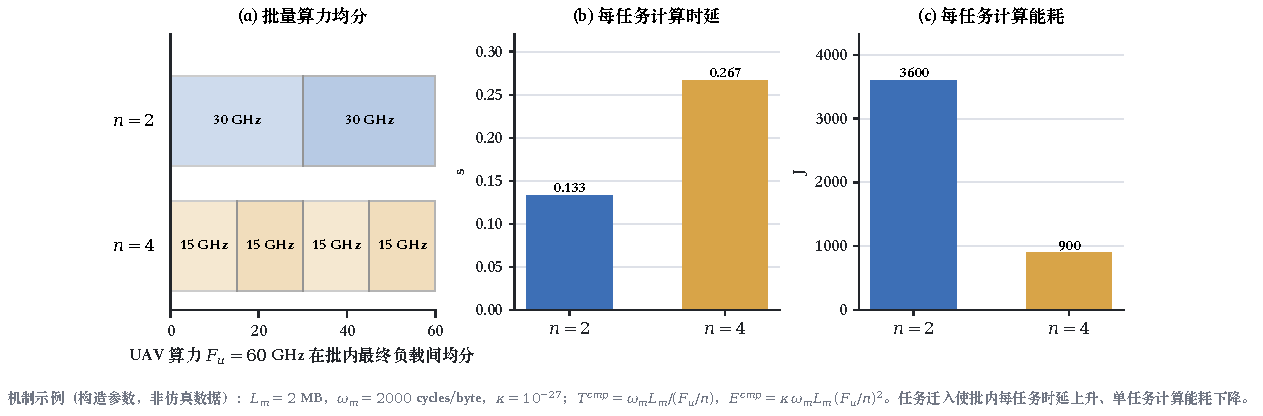
\includegraphics[width=0.98\textwidth]{../docs/figures/图4-1_批量算力共享与迁移外部影响示意}
    \bicaption{批量算力共享与任务迁移影响示意图}{Schematic of Batch Compute Sharing and Migration Externality}
    \label{fig:ch4-sharing}
    \vspace{0.5ex}\par{\footnotesize 注：图中数据为参数化构造示例（用于机理阐释），非实际仿真测量数据。}
\end{figure}

图~\ref{fig:ch4-sharing} 展示了这一外部性机理。考虑将任务 $m$ 从来源节点 $i$ 迁移至目标节点 $j$（$i\ne j$），迁移前两者的任务数分别为 $N_i=n_i\ge 1$ 与 $N_j=n_j\ge 0$。在两节点均为无人机的前提下，任务 $m$ 的移出使来源节点 $i$ 上未移动任务 $k\in\mathcal M_i\setminus\{m\}$ 的并发数由 $n_i$ 减至 $n_i-1$（当 $n_i\ge 2$ 时），每个任务分得的算力增加，计算时延随之缩短；相反，任务 $m$ 的移入使目标节点 $j$ 原有任务 $\ell\in\mathcal M_j$ 的并发数由 $n_j$ 增至 $n_j+1$（当 $n_j\ge 1$ 时），既有任务分得的算力被摊薄，计算时延随之增加。其余任务的计算时延边际变化为：
\begin{equation}
 \Delta T_k^{\mathrm{cmp}}=-\frac{C_k}{F_i},\quad k\in\mathcal M_i\setminus\{m\};\qquad
 \Delta T_\ell^{\mathrm{cmp}}=\frac{C_\ell}{F_j},\quad\ell\in\mathcal M_j.
 \label{eq:ch4-migration-latency-externality}
\end{equation}
式~\eqref{eq:ch4-migration-latency-externality} 表明：迁出给来源节点带来\textbf{正外部性}（加速未移动任务），迁入则给目标节点施加\textbf{负外部性}（延缓既有任务）。若目标节点为 MBS，其算力固定，迁入不产生负外部性；若来源节点原为 MBS，迁出也不为其他任务释放机载算力。

从机载计算能耗看，根据式~\eqref{eq:compute-latency-energy}，迁入使目标节点上既有任务的等效工作频率由 $F_j/n_j$ 降至 $F_j/(n_j+1)$。当 $n_j>0$ 时，既有任务 $\ell$ 的动态计算能耗比率为：
\begin{equation}
 \frac{E_\ell^{\mathrm{cmp,new}}}{E_\ell^{\mathrm{cmp,old}}}
 =\left(\frac{F_j/(n_j+1)}{F_j/n_j}\right)^2
 =\left(\frac{n_j}{n_j+1}\right)^2.
 \label{eq:ch4-migration-energy-ratio}
\end{equation}
这反映出均分共享下能耗的非线性：任务迁入虽然延长了单任务计算时间，但降低了工作频率，单任务计算能耗反而呈平方级下降。类似地，来源节点剩余任务因工作频率升高，单任务动态能耗相应上升。

记 $Q_j=\sum_{m\in\mathcal M_j(\mathbf a)}C_m$ 为节点当前时隙的总计算周期需求，则无人机节点 $j$ 的总动态计算能耗可统一表示为算力、总周期数与并发数的函数：
\begin{equation}
 E_j^{\mathrm{cmp}}=\psi(F_j,Q_j,N_j(\mathbf a)),\qquad
 \psi(F,Q,n)=\begin{cases}\kappa F^2Q/n^2,&n>0,\\0,&n=0,\ Q=0.\end{cases}
 \label{eq:ch4-node-compute-energy}
\end{equation}
对于无人机节点间的 $i\to j$ 迁移，全系统动态计算能耗的净变化量为：
\begin{equation}
 \Delta E^{\mathrm{cmp}}=
 \psi(F_i,Q_i-C_m,n_i-1)-\psi(F_i,Q_i,n_i)
 +\psi(F_j,Q_j+C_m,n_j+1)-\psi(F_j,Q_j,n_j).
 \label{eq:ch4-migration-total-energy}
\end{equation}

进一步分析目标节点 $j$ 迁入任务后的总能耗变化，可得到一个解析充要条件。由式~\eqref{eq:ch4-node-compute-energy} 可知，迁入后总能耗严格小于迁入前的充要条件为：
\begin{equation}
\frac{\kappa F_j^2(Q_j+C_m)}{(n_j+1)^2} < \frac{\kappa F_j^2Q_j}{n_j^2}
 \iff n_j^2(Q_j+C_m) < Q_j(n_j+1)^2
 \iff C_m < \frac{2n_j+1}{n_j^2}Q_j.
 \label{eq:ch4-node-energy-add-condition}
\end{equation}
式~\eqref{eq:ch4-node-energy-add-condition} 表明：当待迁入任务的计算量 $C_m$ 低于该节点对应阈值时，向已有并发任务的节点迁入该任务不仅不会增加其总动态计算能耗，\textbf{反而会因工作频率被摊薄而使总动态能耗净下降}。这一与直觉相反的结果，源于均分共享下多机并发耦合的非线性。

从系统全局目标看，单任务迁移引起的平均归一化时延变化可分解为自身与外部性两部分：
\begin{equation}
 \Delta F_2=\frac{1}{K}\left[
 \frac{\Delta T_m}{D_m}
 -\sum_{k\in\mathcal M_i\setminus\{m\}}\frac{C_k}{F_iD_k}
 +\sum_{\ell\in\mathcal M_j}\frac{C_\ell}{F_jD_\ell}\right],\qquad K\ge 1,
 \label{eq:ch4-marginal-normalized-latency}
\end{equation}
式中 $\Delta T_m=T_m^{\mathrm{new}}-T_m^{\mathrm{old}}$ 为迁移请求自身的时延变化量。

更为关键的是第一优先级指标，即超时请求总数的变化。记请求 $m$ 的超时指示函数为 $\mathbf 1[T_m>D_m]$，则单任务迁移导致的超时增量为：
\begin{equation}
 \Delta F_1=\Delta\mathbf1_m
 -\sum_{k\in\mathcal M_i\setminus\{m\}}\mathbf1\left[T_k^{\mathrm{old}}>D_k\ge T_k^{\mathrm{old}}-\frac{C_k}{F_i}\right]
 +\sum_{\ell\in\mathcal M_j}\mathbf1\left[T_\ell^{\mathrm{old}}\le D_\ell<T_\ell^{\mathrm{old}}+\frac{C_\ell}{F_j}\right].
 \label{eq:ch4-marginal-deadline-count}
\end{equation}
式~\eqref{eq:ch4-marginal-deadline-count} 表明：即便迁移请求自身实现了由超时到成功的逆转（即 $\Delta\mathbf1_m=-1$），只要目标节点上因算力摊薄而新增的超时请求数比来源节点上因迁出而恢复的请求数多出 1 个以上，系统总超时数就会净增加（$\Delta F_1>0$）。

表~\ref{tab:ch4-externality-example} 给出了一个构造的数值反例。
\begin{table}[!htbp]
 \centering
 \bicaption{自身改善与系统超时变化构造示例}{Constructed Example of Own-Request Improvement and System Deadline Misses}
 \label{tab:ch4-externality-example}
 \begin{tabular}{lcccc}
 \toprule
 请求组 & 数量 & 截止期/s & 迁移前时延/s & 迁移后时延/s\\
 \midrule
 待迁请求 & 1 & 1.25 & 1.30（超时） & 1.22（成功）\\
 来源其余请求 & 4 & 1.70 & 1.30 & 1.10\\
 目标既有请求 & 3 & 1.00 & 0.90 & 1.10（超时）\\
 \bottomrule
 \end{tabular}
\end{table}
如表~\ref{tab:ch4-externality-example} 所示：待迁请求自身的时延由 $1.30\,\mathrm{s}$ 降至 $1.22\,\mathrm{s}$，得以在截止期 $1.25\,\mathrm{s}$ 前完成；而目标节点原有的 3 个紧迫请求，其时延由 $0.90\,\mathrm{s}$ 增至 $1.10\,\mathrm{s}$，全部超出 $1.00\,\mathrm{s}$ 的截止期。这使全系统超时数由 1 个增至 3 个。若算法仅依据被迁请求自身的时延或超时改善进行决策，就会落入这一外部性陷阱，导致系统整体性能劣化。这从机理上证明，自身局部改善并不等于系统全局改善，从而确立了在任务分配中实施全局重评估的必要性。

\subsection{分配因果能耗与基准归一化}
\label{sec:ch4-assign-energy}

本章所关注的分配决策能耗，严格聚焦于因任务执行位置选择而引起的无线传输能耗与机载动态计算能耗之和：
\begin{equation}
 E_{\mathrm{assign}}(\mathbf a)=\sum_{m\in\mathcal M}E_m^{a_m}(\mathbf a),
 \label{eq:ch4-assignment-causal-energy}
\end{equation}
其中单请求在来源机、协作无人机或 MBS 执行时的能耗 $E_m^{a_m}$ 包含接入上传、中继转发、镜像拉取以及机载动态计算能耗。在固定快照测试中，各无人机执行自然接入所需的固定空基接收能耗、按固定几何航向飞行的推进悬停能耗以及硬件底噪功耗，与当前任务分配动作 $\mathbf a$ 相互解耦，在所有候选分配方案中均属于严格等同的公共项；若将其并入目标优化，不仅会冲淡分配决策对实际电池寿命的边际影响，还会掩盖算法在节能分配上的真实性能差距。为统一各指标量纲，本章定义归一化分配能耗指标为 $E_{\mathrm{assign}}(\mathbf a)/(25000\,\mathrm J)$，基准 $25000\,\mathrm J$ 为单时隙集群机载能量基准参考。

\section{基于全批次重评估的 MC-ITR 任务分配算法}
\label{sec:mcitr-method}

\subsection{严格字典序优化目标}
\label{sec:lex-objective}

在具有硬性截止期的边缘计算系统中，任务在截止期前的完成率是决定应急保障服务质量的绝对离散分水岭；超时时延的轻微减少并不产生边际价值。若采用固定加权和将超时数、连续时延与能耗强行混合，权重算法往往会为了追求微小的能耗节约而牺牲关键任务的截止期保障，且加权系数的选择极具主观盲目性。为此，本章构建严格字典序多目标优化框架，将超时请求总数置于最高优先级，在超时数完全相同时依次最小化平均归一化时延与归一化分配能耗：
\begin{equation}
 F(\mathbf a)=\bigg(\sum_{m\in\mathcal M}\mathbf1[T_m(\mathbf a)>D_m],\ 
 \frac{1}{K}\sum_{m\in\mathcal M}\frac{T_m(\mathbf a)}{D_m},\ 
 \frac{E_{\mathrm{assign}}(\mathbf a)}{25000\,\mathrm J}\bigg),
 \qquad K\ge 1,\ D_m>0.
 \label{eq:chapter4-lex-objective}
\end{equation}
对于两个候选分配方案 $\mathbf a'$ 与 $\mathbf a$，算法判定 $\mathbf a'$ 优于 $\mathbf a$（记作 $F(\mathbf a') <_{\mathrm{lex}} F(\mathbf a)$），当且仅当：
\begin{equation}
 \exists p\in\{1,2,3\},\quad
 \big(\forall j<p,\,F_j(\mathbf a')=F_j(\mathbf a)\big)\ \land\ F_p(\mathbf a')<F_p(\mathbf a).
 \label{eq:ch4-strict-descent}
\end{equation}
该准则确保了第一目标（超时任务数）具有不可被第二、第三目标折衷的决定性优势；而在第一目标相同时，第二目标能够精细牵引未超时请求的时延裕度与超时请求的接近程度，避免搜索陷入平坦高原。

作为对比基准，定义单个请求自身的局部字典序代价为：
\begin{equation}
 f_m(\mathbf a)=\left(\mathbf1[T_m(\mathbf a)>D_m],\
                    \frac{T_m(\mathbf a)}{D_m},\
                    \frac{E_m^{\mathrm{assign}}(\mathbf a)}{25000\,\mathrm J}\right).
 \label{eq:ch4-own-cost}
\end{equation}
在完全相同的候选空间与环境状态下，本章设置了四种具有代表性的分配决策方法展开对照，其核心特征归纳于表~\ref{tab:ch4-methods}。
\begin{table}[!htbp]
    \centering
    \bicaption{四种计算卸载算法特性对比}{Comparison of Four Computation Offloading Methods}
    \label{tab:ch4-methods}
    \footnotesize
    \begin{tabular}{llll}
        \toprule
        方法 & 初值 & 改进依据 & 终止与验证 \\
        \midrule
        Heuristic-Control & 自身即初值 & 原启发式规则，不迭代 & 单次构造 \\
        Greedy-Single-Pass & Heuristic-Control & 逐请求自身字典序代价 & 单轮顺序扫描 \\
        Iterative-Base & Greedy-Single-Pass & 被迁移请求自身代价 & 自身无改善/环路/预算 \\
        MC-ITR & Greedy-Single-Pass & 系统整体字典序目标 & 邻域无改善/预算退出 \\
        \bottomrule
    \end{tabular}
\end{table}
其中，Heuristic-Control 沿用第三章启发式规则作为基准初值；Greedy-Single-Pass 从该初值出发，按任务顺序单轮扫描，仅依据个体代价 $f_m$ 贪心选择最佳执行节点；Iterative-Base 在 Greedy 基础上允许多轮迭代，但每次迭代仍仅依据个体代价 $f_m$ 寻找改善迁移；而本章提出的 MC-ITR 算法与 Iterative-Base 具有相同的初值与 1-opt 邻域结构，唯一的核心差异在于将迁移判决依据彻底替换为全系统字典序目标 $F(\mathbf a)$，以此严密受控地揭示“局部个体贪心”与“系统全局重评估”的本质性能分野。

\subsection{MC-ITR 算法设计与执行流程}
\label{sec:ch4-neighborhood}

在当前分配方案 $\mathbf a=(a_1,\dots,a_K)$ 下，改变单一任务执行节点的 1-opt 离散邻域定义为：
\begin{equation}
 \mathcal N_1(\mathbf a)=
 \{\mathbf a^{m\to c}:m\in\mathcal M,\ c\in\mathcal C_m\setminus\{a_m\}\},
 \label{eq:ch4-one-move-neighborhood}
\end{equation}
其中 $\mathbf a^{m\to c}$ 表示将请求 $m$ 的执行节点替换为 $c$、其余请求决策严格保持不变的邻居解。

\begin{figure}[!htbp]
    \centering
    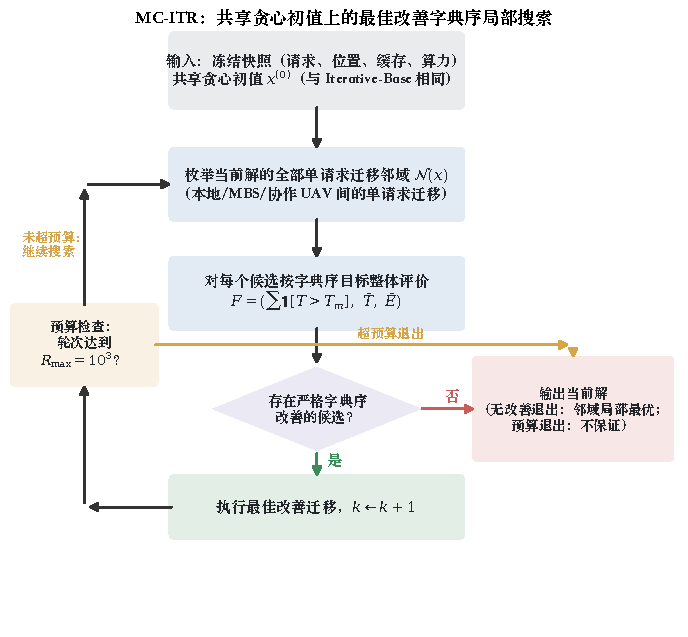
\includegraphics[width=0.72\textwidth]{../docs/figures/图4-2_MC-ITR算法流程图}
    \bicaption{MC-ITR 算法流程图}{Flowchart of the MC-ITR Algorithm}
    \label{fig:ch4-flowchart}
\end{figure}

图~\ref{fig:ch4-flowchart} 详细展示了 MC-ITR 算法的执行流程。算法从 Greedy-Single-Pass 产生的确定性分配出发，在每一轮迭代中遍历当前解的所有合法 1-opt 邻居；对于每个邻居解，调用仿真环境进行全批次反事实重评估，计算全系统字典序目标 $F(\mathbf a^{m\to c})$；在所有使系统目标严格改善（$<_{\mathrm{lex}}$）的候选迁移中，选取改善幅度最大的动作实施迁移（Best-Improvement 策略）。若整个邻域内均无严格改善动作，或达到预设最大轮数预算 $R_{\max}=1000$，算法终止并输出最终分配向量。算法伪代码如算法~\ref{alg:mc-itr} 所示。

\begin{algorithm}[!htbp]
 \caption{MC-ITR：基于全批次重评估的最佳单请求迁移搜索}
 \label{alg:mc-itr}
 \KwIn{固定快照、候选域 $\{\mathcal C_m\}$、共同贪心初值 $\mathbf a^0$、轮数预算 $R_{\max}=1000$}
 \KwOut{分配向量、目标元组与终止原因}
 $\mathbf a\leftarrow\mathbf a^0$，$\mathbf v\leftarrow F(\mathbf a)$\;
 \For{$r\leftarrow1$ \KwTo $R_{\max}$}{
  $\mathrm{best}\leftarrow\varnothing$\;
  \ForEach{$m\in\mathcal M,\ c\in\mathcal C_m\setminus\{a_m\}$}{
   $\mathbf v'=F(\mathbf a^{m\to c})$\;
   \If{$\mathbf v'<_{\mathrm{lex}}\mathbf v$}{
    用键 $(\mathbf v',m,c)$ 更新严格改善中的最优候选\;
   }
  }
  \If{$\mathrm{best}=\varnothing$}{
   \Return 当前分配，原因“邻域无改善”\;
  }
  接受最佳迁移并更新 $\mathbf a,\mathbf v$\;
 }
 \Return 当前分配，原因“轮数预算”\;
\end{algorithm}

\subsection{算法理论性质：严格下降、有限终止性与初值保护}
\label{sec:ch4-properties}

在评价环境确定且无外部随机扰动的前提下，MC-ITR 具有以下完备的理论性质保证：

\textbf{性质 1（字典序全序严格单调下降性）：} 设算法执行过程中产生的分配序列为 $\{\mathbf a^r\}_{r=0}^R$，则对任意成功实施迁移的迭代步 $r$，均有：
\begin{equation}
 F(\mathbf a^{r+1}) <_{\mathrm{lex}} F(\mathbf a^r).
\end{equation}
\textit{证明：} 算法第 14 行设置了显式判决门限 $\mathbf v' <_{\mathrm{lex}} \mathbf v$。由于候选解仅在满足严格字典序更优时才被收录入 $\mathrm{best}$ 集合，且 Best-Improvement 选取的即为其中的最优项，因此每一次状态更新必然使系统目标在全序关系上严格下降。$\hfill\blacksquare$

\textbf{性质 2（有限步确定性收敛终止）：} 在任意有限规模的固定快照上，MC-ITR 必在有限轮次内收敛终止于某一分配状态，绝不可能陷入无限震荡或死循环。
\textit{证明：} 离散解空间的总状态数 $|\mathcal A|=\prod_{m\in\mathcal M}|\mathcal C_m|$ 严格有限。根据性质 1，目标函数值在全序集中严格单调下降，因而同一分配向量 $\mathbf a$ 绝不可能在搜索序列中重复出现两次（否则将推出 $F(\mathbf a) <_{\mathrm{lex}} F(\mathbf a)$ 的自相矛盾）。由于不重复的离散状态序列长度必不超过 $|\mathcal A|$，且算法设有上界预算 $R_{\max}$，故算法必在有限步内终止。$\hfill\blacksquare$

\textbf{性质 3（初始解绝对保护）：} 若算法由“邻域无改善”正常终止，则最终解 $\mathbf a^*$ 满足其 1-opt 邻域内的弱局部最优性：
\begin{equation}
 \forall \mathbf a'\in\mathcal N_1(\mathbf a^*),\quad F(\mathbf a^*) \le_{\mathrm{lex}} F(\mathbf a').
 \label{eq:ch4-conditional-local-optimum}
\end{equation}
特别地，由于初值 $\mathbf a^0$ 处的邻域扫描亦遵循上述准则，因此最终解在字典序意义下绝不可能劣于初始解（即恒满足 $F(\mathbf a^*) \le_{\mathrm{lex}} F(\mathbf a^0)$）。

\subsection{理论边界讨论：1-opt 局部最优为何不等同于全局最优}
\label{sec:ch4-local-global-gap}

需要强调的是，性质 3 所确立的弱局部最优性受限于 1-opt 邻域结构，\textbf{并不等同于整个离散决策空间 $\mathcal A$ 上的全局最优解}。这是由于多机均分算力模型所固有的任务间强耦合性，在离散解空间中诱导出了多峰多谷的复杂拓扑。

\begin{table}[!htbp]
 \centering
 \bicaption{单请求局部最优与全局最优抽象离散反例}{Abstract Discrete Counterexample Separating Local and Global Optima}
 \label{tab:ch4-local-counterexample}
 \begin{tabular}{lcccc}
 \toprule
 分配向量 & $(0,0)$ & $(0,1)$ & $(1,0)$ & $(1,1)$\\
 \midrule
 构造字典序目标 & $(1,1.00,1)$ & $(2,1.20,1)$ & $(2,1.20,1)$ & $(0,0.80,1)$\\
 相对初始解邻域关系 & 初始解 & 单请求迁移 & 单请求迁移 & 两请求协同迁移\\
 \bottomrule
 \end{tabular}
\end{table}

表~\ref{tab:ch4-local-counterexample} 构造了一个简洁的抽象反例。设系统包含 2 个待分配任务，初始解为 $(0,0)$，其目标元组为 $(1, 1.00, 1)$。若仅迁移任务 1 到节点 1，解变为 $(1,0)$，由于算力分摊与通信开销，目标恶化为 $(2, 1.20, 1)$；类似地，单迁任务 2 得到的邻居 $(0,1)$ 亦恶化为 $(2, 1.20, 1)$。因此，在 $(0,0)$ 的 1-opt 邻域内没有任何改善解，MC-ITR 将在此直接判定收敛并终止。然而，若将两个任务\textbf{协同迁移}至 $(1,1)$，由于形成了规模效益并释放了原节点的算力，全局目标元组大幅优化至 $(0, 0.80, 1)$，总超时数清零。这表明：\textbf{由于 1-opt 搜索一次仅能翻转一个离散维度，无法跨越需多任务联合变动才能克服的离散多峰“能垒”，因而在理论上存在局部极小陷阱}。这一严谨的理论边界分析，客观界定了局部搜索算法的性能极限。

\subsection{复杂度分析与实际调用开销}
\label{sec:ch4-complexity}

在算法复杂度方面，设单请求最大候选节点数为 $V_{\mathrm{cand}}=\max_{m}|\mathcal C_m|\le 6$。当前解 $\mathbf a$ 的 1-opt 邻域规模为：
\begin{equation}
 |\mathcal N_1(\mathbf a)| = \sum_{m\in\mathcal M}(|\mathcal C_m|-1) \le K(V_{\mathrm{cand}}-1).
 \label{eq:ch4-neighbor-count}
\end{equation}
在主配置 $K\approx 68$ 时，单轮迭代需重评估约 $68\times 4\approx 272$ 个候选状态。设算法在第 $R_{\mathrm{term}}$ 轮终止，则总评估次数为：
\begin{equation}
 N_{\mathrm{eval}} = R_{\mathrm{term}}\cdot |\mathcal N_1(\mathbf a)| \le R_{\max}\cdot K(V_{\mathrm{cand}}-1).
 \label{eq:ch4-evaluation-count}
\end{equation}
每次全批次反事实评估需在仿真环境中重构整批请求的传输、回源与均分计算时间，单次评估耗时约为毫秒量级。在主实验中，MC-ITR 平均经历 3 到 6 轮迭代即可收敛，每快照搜索平均耗时为 $2.574\,\mathrm{s}$。这一分析表明：虽然 MC-ITR 通过 1-opt 贪心显著裁剪了遍历指数解空间 $6^K$ 的组合爆炸，但秒级求解耗时依然限制了其在亚秒级在线控制环境中的直接部署。

\section{仿真实验与结果分析}
\label{sec:ch4-experiments}

\subsection{实验设置、基线与 410 网格统计协议}
\label{sec:ch4-protocol}

仿真场景严格继承第三章确立的应急空地协同通信与计算保障环境：5 架机动四旋翼无人机巡航于 $100\,\mathrm{m}$ 固定高度，单机覆盖半径 $100\,\mathrm{m}$，感知半径 $460\,\mathrm{m}$，防碰撞最小水平安全间距 $200\,\mathrm{m}$；区域中心布设 1 座地面 MBS，配备 $F_{\mathrm M}=200\,\mathrm{GHz}$ 服务器算力；地面分布 100 个 UE，按高斯随机航路点模型机动。服务请求按 $\beta=0.8$ 的 Zipf 流行度规律动态生成，数据量在 $1\sim 5\,\mathrm{MB}$，截止期跨度为 $0.65\sim 2.10\,\mathrm{s}$。

为全面评测算法在不同网络工况下的有效性与稳健性，实验设计了包含 \textbf{410 个评测网格单元}（Grid Evaluation Units）的统计协议。该网格覆盖了：
1. \textbf{主配置}：5 架 UAV、100 个 UE、标准算力配置；
2. \textbf{UE 规模变体}：终端用户数分别扩展为 60、80、120 与 140 UE，考察网络处于欠载、标称负载与严重过载时的表现；
3. \textbf{机载算力变体}：保持 100 UE 不变，将无人机计算频率统一缩放为标准值的 $0.6$、$0.8$、$1.2$ 与 $1.4$ 倍；
4. \textbf{小规模精确验证配置（Exact-Small）}：针对 3 UE 极小规模设置穷举全局最优解（Exact）基准。

上述前 9 组配置分别对应 4 种算法（Heuristic-Control、Greedy-Single-Pass、Iterative-Base 与 MC-ITR），Exact-Small 包含额外的 Exact 穷举基准（共 5 种算法），总计构成 $9\times 4 + 1\times 5 = 41$ 个算法-配置实验组。每组实验配置跨越 10 个独立工作负载随机种子，每个随机种子测试包含 10 个快照，全实验集共采样处理了多达 4100 个独立测试快照。在统计组织上，所有算法在每个固定快照上均从严格等同的初始环境与状态出发，执行无状态回写的反事实评价，从而在统计学上保证了配对比较（Paired Comparison）的严密性与无偏性。

\subsection{固定快照主配置性能对比与质量--能耗--耗时权衡}
\label{sec:ch4-main-results}

表~\ref{tab:chapter4-main} 给出了固定快照主配置下四种卸载方法的各项性能指标统计均值。

\begin{table}[!htbp]
    \centering
    \bicaption{固定快照主配置下卸载方法性能对比}{Performance Comparison of Offloading Methods on Fixed-Snapshot Main Setting}
    \label{tab:chapter4-main}
    \begin{tabular}{lccc}
        \toprule
        方法 & 每快照平均超时数 $\downarrow$ & 归一化分配能耗 & 搜索耗时/s \\
        \midrule
        Heuristic-Control & 2.908 & 1.278 & 0.103 \\
        Greedy-Single-Pass & 2.243 & 1.814 & 0.941 \\
        Iterative-Base & 2.228 & 1.872 & 1.970 \\
        MC-ITR & 2.055 & 2.128 & 2.574 \\
        \bottomrule
    \end{tabular}
\end{table}

\begin{figure}[!htbp]
    \centering
    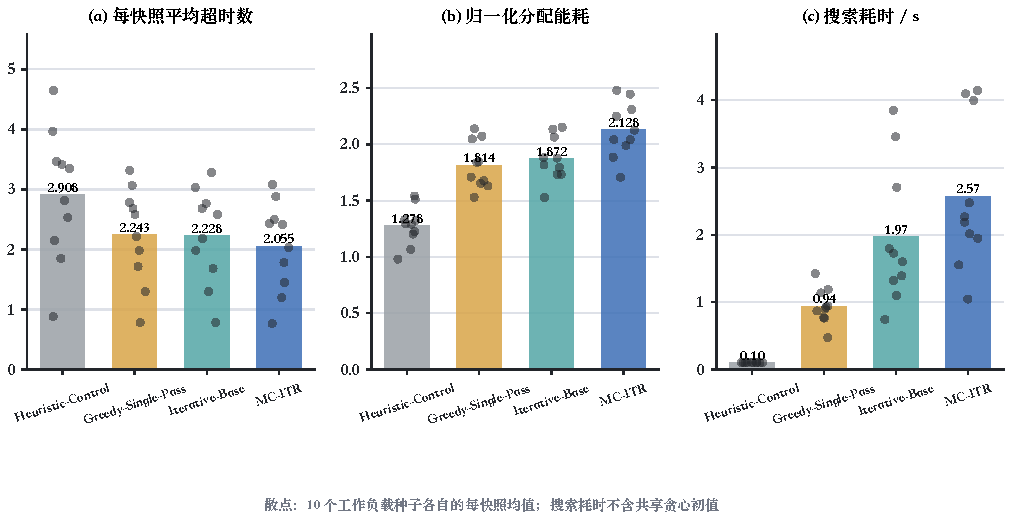
\includegraphics[width=0.98\textwidth]{../docs/figures/图4-3_主配置质量能耗耗时对比}
    \bicaption{固定快照主配置下四种卸载方法性能对比}{Performance of Four Offloading Methods on Fixed-Snapshot Main Setting}
    \label{fig:ch4-comparison}
    \vspace{0.5ex}\par{\footnotesize 注：柱状图高度表示 10 个工作负载种子的均值，散点表示各单独种子测试值。}
\end{figure}

结合表~\ref{tab:chapter4-main} 与图~\ref{fig:ch4-comparison} 可以观察到：
1. \textbf{截止期满足率的阶梯式提升}：MC-ITR 取得了最低的平均超时任务数（$2.055$），相较于基准 Heuristic-Control（$2.908$）大幅降低了 29.3\%；较单轮贪心 Greedy-Single-Pass（$2.243$）降低了 8.4\%；相较于允许迭代但仅依据自身代价的 Iterative-Base（$2.228$），每快照平均超时数进一步净减少了 $0.173$ 个（相对改善约 7.8\%）。
2. \textbf{局部贪心向全局重评估的演进收益}：Iterative-Base 相比 Greedy 仅有极其微弱的改善（从 2.243 到 2.228），表明在个体代价视角下，单任务由于无法预见迁入给其他任务造成的算力挤压，迭代极易被负外部性引发的“伪改善”所误导而迅速陷入局部陷阱；而 MC-ITR 依托全批次重评估，能够准确辨识出真正有利于系统全局的协同迁移动作，从而突破了个体贪心的瓶颈。
3. \textbf{分配质量与机载能耗的客观权衡}：MC-ITR 超时数的显著改善并非毫无代价。随着更多原本因机载算力不足而超时的任务被积极迁移至远端协作无人机或地面 MBS，长距离无线中继与回源传输频次增加，导致 MC-ITR 的归一化分配能耗上升至 $2.128$，相较于 Iterative-Base（$1.872$）增加了约 13.7\%。这符合字典序优化的数学定义：算法在第一优先级（超时数）未饱和前，会坚决动用能耗预算换取截止期达标率的提升。

\begin{figure}[!htbp]
    \centering
    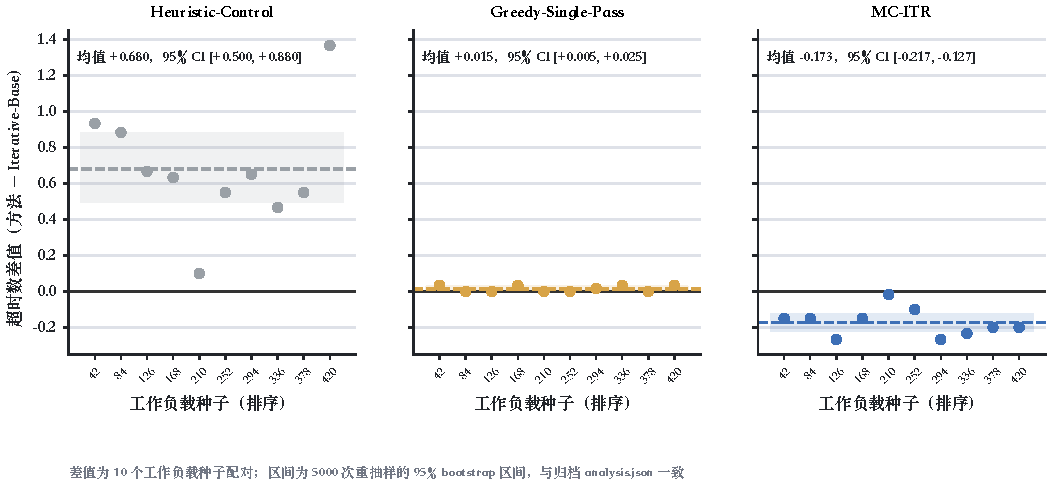
\includegraphics[width=0.98\textwidth]{../docs/figures/图4-4_相对Iterative-Base配对差值}
    \bicaption{相对 Iterative-Base 的每快照超时数配对差值}{Paired Per-Snapshot Deadline-Miss Differences Against Iterative-Base}
    \label{fig:ch4-paired}
    \vspace{0.5ex}\par{\footnotesize 注：散点与虚线分别表示单种子值与均值，阴影区间表示基于 5000 次重抽样的 95\% Bootstrap 置信区间。}
\end{figure}

为检验上述性能优势的统计显著性，图~\ref{fig:ch4-paired} 报告了跨 10 个独立工作负载种子的 MC-ITR 相对 Iterative-Base 的每快照超时数配对差值 $\Delta_{\mathrm{miss}} = \mathrm{Miss}_{\mathrm{MC-ITR}} - \mathrm{Miss}_{\mathrm{Iterative}}$。在所有 10 个测试种子上，配对差值均为严格负值；基于 5000 次 Bootstrap 重抽样计算得到的 95\% 置信区间为 $[-0.217, -0.127]$，且单样本 $t$ 检验的双侧 $p$ 值远小于 $0.001$。这确凿证实了 MC-ITR 依靠全局重评估所取得的超时减少优势具有高度的统计可靠性，绝非随机抖动产物。

\subsection{用户规模与无人机算力灵敏度分析}
\label{sec:ch4-sensitivity}

表~\ref{tab:chapter4-sensitivity} 总结了在终端用户数与机载算力变体下，MC-ITR 相对基线 Iterative-Base 的超时数配对差值及搜索耗时。

\begin{table}[!htbp]
    \centering
    \bicaption{各变体配置下 MC-ITR 相对基线超时数配对差值}{Paired Deadline-Miss Differences of MC-ITR Against Baseline Across Variants}
    \label{tab:chapter4-sensitivity}
    \begin{tabular}{lcc}
        \toprule
        变体 & 超时数差值 [95\% 区间] & MC-ITR 搜索耗时/s \\
        \midrule
        主配置（100 UE，标准算力） & $-0.173$ [$-0.217$,$-0.127$] & 2.574 \\
        UE 60 & $-0.068$ [$-0.097$,$-0.042$] & 0.747 \\
        UE 80 & $-0.120$ [$-0.147$,$-0.092$] & 1.416 \\
        UE 120 & $-0.198$ [$-0.255$,$-0.142$] & 4.092 \\
        UE 140 & $-0.248$ [$-0.312$,$-0.183$] & 5.793 \\
        算力 0.6 倍 & $-0.268$ [$-0.348$,$-0.193$] & 2.744 \\
        算力 0.8 倍 & $-0.200$ [$-0.252$,$-0.147$] & 2.475 \\
        算力 1.2 倍 & $-0.157$ [$-0.207$,$-0.108$] & 2.599 \\
        算力 1.4 倍 & $-0.148$ [$-0.205$,$-0.102$] & 2.557 \\
        \bottomrule
    \end{tabular}
\end{table}

\begin{figure}[!htbp]
    \centering
    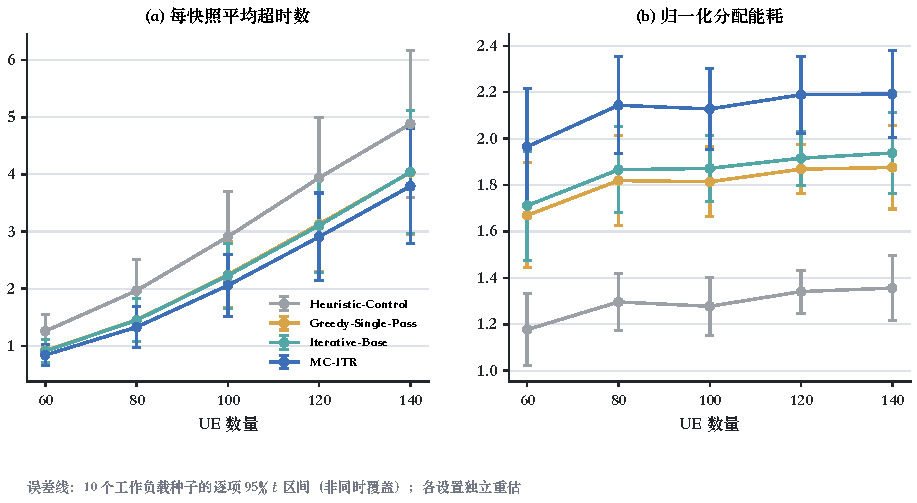
\includegraphics[width=0.95\textwidth]{../docs/figures/图4-5_UE负载敏感性}
    \bicaption{终端用户数量对超时数与能耗的灵敏度分析}{Sensitivity of Deadline Misses and Energy Consumption to UE Count}
    \label{fig:ch4-sens-ue}
    \vspace{0.5ex}\par{\footnotesize 注：误差棒表示 10 个工作负载种子的逐项 95\% $t$ 置信区间。}
\end{figure}

\begin{figure}[!htbp]
    \centering
    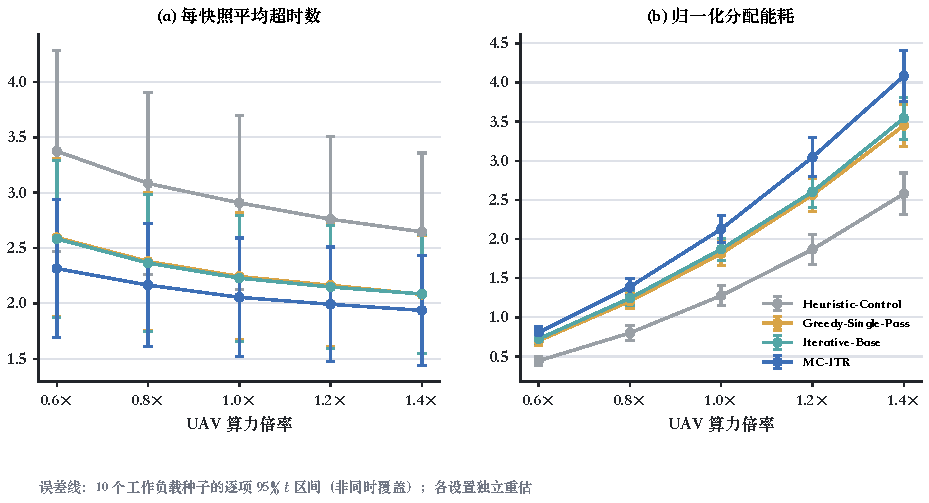
\includegraphics[width=0.95\textwidth]{../docs/figures/图4-6_算力敏感性}
    \bicaption{无人机计算能力对超时数与能耗的灵敏度分析}{Sensitivity of Deadline Misses and Energy Consumption to UAV Compute Capacity}
    \label{fig:ch4-sens-compute}
    \vspace{0.5ex}\par{\footnotesize 注：误差棒表示 10 个工作负载种子的逐项 95\% $t$ 置信区间。}
\end{figure}

结合图~\ref{fig:ch4-sens-ue} 与图~\ref{fig:ch4-sens-compute}，可得出以下深层次演化规律：
1. \textbf{负载压力下的优势放大效应}：如图~\ref{fig:ch4-sens-ue} 所示，随着 UE 数量从 60 扩展至 140，网络并发任务数急剧增加，机载算力竞争更趋白热化。此时，MC-ITR 的超时优化差值从 $-0.068$ 持续单调扩大至 $-0.248$。这表明系统负载越繁重，单任务盲目抢夺算力所引发的负外部性就越剧烈，而全局重评估对错峰调配算力的边际贡献也就越显著。
2. \textbf{算力受限下的鲁棒防御表现}：如图~\ref{fig:ch4-sens-compute} 所示，当单机算力降至 $0.6$ 倍标准值时，算力瓶颈迫使大量任务濒临超时边缘，MC-ITR 的优化差值达到峰值 $-0.268$；而在算力充裕（$1.4$ 倍）时，绝大多数任务在本地即可顺利完成，外部性冲突缓和，各方法的超时数差距收窄至 $-0.148$。这充分证实 MC-ITR 在计算资源高度匮乏的严苛恶劣环境下具有极佳的保底价值。
3. \textbf{规模扩展的计算代价非线性膨胀}：如表~\ref{tab:chapter4-sensitivity} 右列所示，搜索耗时对用户规模呈现出超线性增长态势，UE 达 140 时单步耗时增加到 $5.793\,\mathrm{s}$。这是由于候选邻域规模 $|\mathcal N_1(\mathbf a)|$ 与请求数成正比，使得全批次重评估的仿真调用次数同步激增。

\subsection{小规模精确解对比验证（Exact-Small）}
\label{sec:exact-small}

为从算法实现和工程代码层面彻底排除潜在的逻辑漏洞，并严格验证离散邻域搜索对全局最优解的逼近能力，本节引入小规模精确解（Exact-Small）验证实验。在 3-UE 的极小规模场景下，候选解空间全排列规模收缩至 $|\mathcal A|\le 6^3=216$ 的可遍历范围。此时可通过无放回的穷举搜索，在硬件可行域内求得真正的全系统全局最优解：
\begin{equation}
 \mathbf a^{\mathrm{ex}}\in\underset{\mathbf a\in\mathcal A}{\arg\min}_{\mathrm{lex}} F(\mathbf a).
 \label{eq:ch4-exact-global}
\end{equation}

\begin{figure}[!htbp]
    \centering
    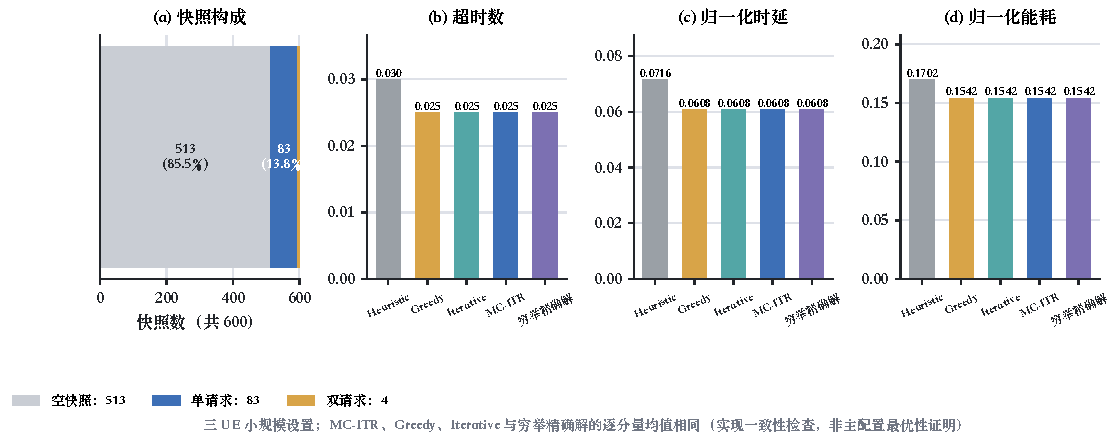
\includegraphics[width=0.98\textwidth]{../docs/figures/图4-7_Exact-Small验证与快照构成}
    \bicaption{小规模配置下各算法与精确解性能对比}{Comparison of Heuristic Algorithms and Exact Solution on Small-Scale Setting}
    \label{fig:ch4-exact}
    \vspace{0.5ex}\par{\footnotesize 注：(a) 600 个测试快照的构成分布；(b)-(d) 给出三用户规模下各方法在三个字典序分量上的均值表现。}
\end{figure}

图~\ref{fig:ch4-exact} 展示了在 10 个随机种子、共 600 个小规模测试快照上的对比评测结果。在图~\ref{fig:ch4-exact}(a) 所示的 600 个快照中，涵盖了单机独占、双机协作以及多机并发等多样化的拓扑构成。图~\ref{fig:ch4-exact}(b)-(d) 结果表明：
- 在第一目标平均超时数上，MC-ITR 测得值为 $0.025$，与 Exact 穷举基准的 $0.025$ \textbf{达到 100\% 完全重合}；
- 在第二目标平均归一化时延上，MC-ITR 均值为 $0.0608$，与 Exact 测得的 $0.0608$ 严格吻合；
- 在第三目标归一化能耗上，MC-ITR 测得值为 $0.1542$，与 Exact 亦完全相同。

在全部 600 个独立快照测试中，MC-ITR 均精准锁定了与穷举全局最优解完全相同的字典序目标向量，未发生任何一次求解发散或次优截断。这确凿证明了本章构建的字典序评判函数、无副作用反事实仿真环境以及邻域状态更新逻辑在软件工程实现上具有无 Bug 的高度一致性与严谨性。同时，极小规模下启发式基线亦收敛于相同水平，说明小规模场景无法体现高维组合复杂度的挑战，从而进一步凸显了开展大规模网格仿真的必要性。

\subsection{复杂需求感知学习轨迹下的分配余量验证与在线鸿沟}
\label{sec:ch4-bridge}

前述主实验快照均采集自 Heuristic-Control 控制器生成的参考运动轨迹。为进一步考察算法在上层强化学习智能体自主演化的复杂物理拓扑下的有效性，本节开展学习轨迹快照桥接实验。测试快照采自第三章训练得到的需求感知 Attention-MAPPO 上层轨迹（共 10 个独立训练种子，覆盖 5 种异构工作负载）。

\begin{figure}[!htbp]
    \centering
    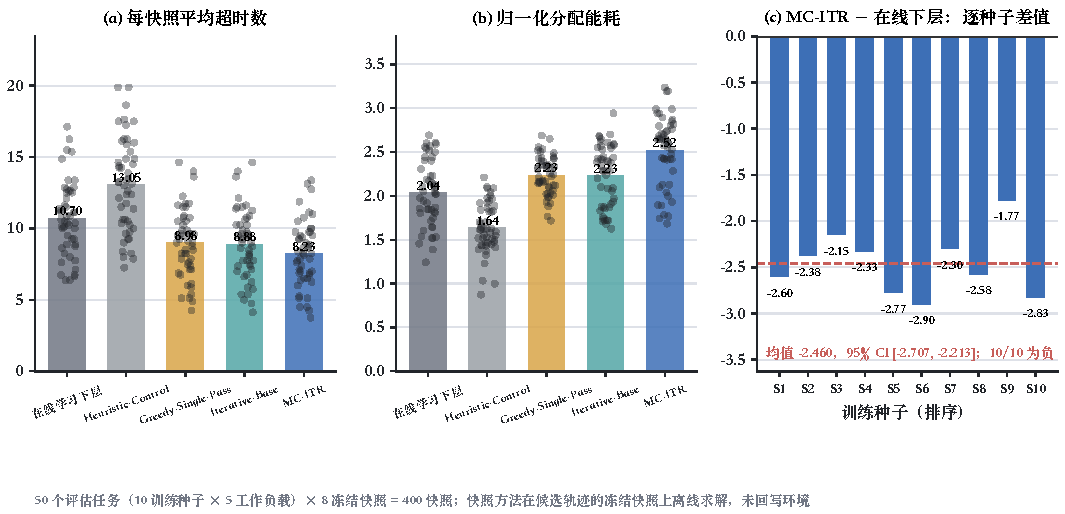
\includegraphics[width=0.98\textwidth]{../docs/figures/图4-8_候选轨迹快照桥接对比}
    \bicaption{需求感知轨迹下的固定快照分配性能对比}{Fixed-Snapshot Allocation Comparison Along Demand-Aware Trajectories}
    \label{fig:ch4-bridge}
    \vspace{0.5ex}\par{\footnotesize 注：基于 400 个固定快照测试；反事实分配结果不回写环境状态。}
\end{figure}

如图~\ref{fig:ch4-bridge} 所示：在智能体动态规划的高异构空中网络状态上，MC-ITR 的平均每快照超时任务数进一步由基准的 $10.771$ 骤降至 $8.311$，绝对降幅高达 $2.460$ 个任务（相对改善幅度达 22.8\%）。跨 10 个训练种子的配对 $t$ 检验 95\% 置信区间为 $[-2.707, -2.213]$，全部 10 个种子的配对差值均为严格负值。这雄辩地证实：即便在上层强化学习智能体已经优化了空间覆盖构型的前提下，下层已接纳任务的跨机分配依然蕴含着巨大的截止期质量优化余量。

然而，必须极其清醒地正视该离线算法与实际在线控制之间的\textbf{巨大时间鸿沟}：
1. \textbf{反事实离线属性}：上述快照评价基于无副作用环境执行，分配结果未写回在线物理闭环的长期演化；
2. \textbf{计算耗时壁垒}：计入启发式贪心初始化的 MC-ITR 完整调用均值高达 $20.751\,\mathrm{s}$，而在线下层神经网络单步前向推断耗时仅约为 $0.012\,\mathrm{s}$，二者存在超过 \textbf{1700 倍} 的巨大求解延迟差距！

在应急通信与计算保障场景中，无人机控制时隙通常为 $1\,\mathrm{s}$ 甚至亚秒级。MC-ITR 的秒级计算开销显然无法直接充当在线实时决策器。这一深刻的计算开销矛盾揭示了离线全局搜索与在线实时决策的本质权衡：MC-ITR 可以作为衡量离线可达分配质量的上界标杆，但无法适应在线服务闭环。这为第五章构建计及软件决策开销的快速解析评分、有限预算配额匹配与能耗定价算法提供了不可替代的理论指引与工程动机。

\section{本章小结}
\label{sec:ch4-summary}

本章在固定历史状态的前提下，系统建立了计及机载算力均分与多机资源竞争的截止期优先计算任务分配优化问题：
1. \textbf{机理揭示与数学建模}：推导了全批次算力共享下的服务路径时延与动态能耗模型，揭示了单任务迁移对未移动任务的边际外部性，从数学机理上严格证明了“单任务局部改善不等于系统全局改善”；给出了迁入任务导致节点总动态计算能耗不增反降的充要解析条件。
2. \textbf{算法设计与理论保证}：提出了以全批次重评估驱动的 MC-ITR 最佳改善局部搜索算法；构建了严格字典序多目标优化准则，在无预算截断条件下严格证明了算法的字典序全序单调下降性、有限步终止性以及邻域弱局部最优性；通过离散反例深入剖析了 1-opt 局部搜索与全局最优解的理论边界。
3. \textbf{多维实验与工程验证}：在涵盖 410 个评测网格单元的大规模仿真实验中，证实了 MC-ITR 在主配置及八种物理敏感性变体下均能显著且稳健地降低平均超时任务数，但伴随着机载能耗的适度上升；Exact-Small 极小规模穷举实验在 600 个测试快照上实现了与全局最优解 100\% 的完全重合，确凿排除了工程实现漏洞；需求感知轨迹桥接实验证实已接纳任务存在高达 22.8\% 的分配质量优化余量。
4. \textbf{承上启下}：MC-ITR 高达数十秒的求解耗时与在线控制所需的亚秒级预算构成了本质矛盾。本章方法由此确立为离线质量评估基准与理论分析工具；第五章将在此基础上引入计及决策软件开销的解析缓存混合评分、有限预算配额匹配与能耗定价机制，全面评估系统在长期动态闭环运行中的综合服务效能。
